\documentclass[12pt,a4paper]{article}
\usepackage[a4paper, margin=0.8in, headheight=14pt]{geometry}
\usepackage{fontspec}
\usepackage{unicode-math}
\setmainfont{TeX Gyre Pagella}
\setmonofont[Scale=0.88]{TeX Gyre Cursor}
\setmathfont{Latin Modern Math}

\usepackage{xcolor}
\usepackage{colortbl}
\usepackage{titlesec}
\usepackage{enumitem}
\usepackage{tabularx}
\usepackage{booktabs}
\usepackage{array}
\usepackage{amsmath}
\allowdisplaybreaks
\usepackage{tikz}
\usetikzlibrary{shapes.geometric, arrows.meta, positioning, calc, fit, decorations.pathreplacing, patterns}
\usepackage{tcolorbox}
\tcbuselibrary{skins, breakable}
\usepackage{hyperref}
\usepackage{fancyhdr}
\usepackage{graphicx}
\usepackage{microtype}
\hyphenpenalty=10000
\exhyphenpenalty=10000
\sloppy
\usepackage{caption}
\usepackage{setspace}
\usepackage{multirow}
\usepackage{tocloft}

% ─── Q&A helper ────────────────────────────────────────────────────────────────
\newcommand{\Q}[1]{\textbf{#1}\par\noindent\ignorespaces}

% ─── Colour Palette ────────────────────────────────────────────────────────────
\definecolor{myred}{RGB}{196,30,58}
\definecolor{mydark}{RGB}{30,30,50}
\definecolor{mygreen}{RGB}{14,120,80}
\definecolor{myteal}{RGB}{0,130,140}
\definecolor{myamber}{RGB}{220,130,20}
\definecolor{mypurple}{RGB}{90,40,140}
\definecolor{mygray}{RGB}{248,249,251}
\definecolor{mgframe}{RGB}{215,220,230}
\definecolor{watermark}{RGB}{145,150,170}
\definecolor{hdrred}{RGB}{250,232,235}
\definecolor{hdrgreen}{RGB}{220,244,233}
\definecolor{hdrteal}{RGB}{220,242,244}
\definecolor{hdramber}{RGB}{253,242,215}
\definecolor{hdrpurple}{RGB}{238,228,255}
\definecolor{hdrgray}{RGB}{238,240,245}
\definecolor{rowalt}{RGB}{250,251,253}

% ─── Section Formatting ────────────────────────────────────────────────────────
\titleformat{\section}
  {\large\bfseries\color{myred}}{\thesection.}{0.5em}{}
  [\vspace{1pt}{\color{myred}\rule{\linewidth}{0.8pt}}]
\titleformat{\subsection}
  {\normalsize\bfseries\color{myteal}}{\thesubsection}{0.5em}{}
\titlespacing*{\section}{0pt}{18pt}{7pt}
\titlespacing*{\subsection}{0pt}{11pt}{4pt}

% ─── Paragraph ─────────────────────────────────────────────────────────────────
\setlength{\parindent}{0pt}
\setlength{\parskip}{4pt}

% ─── TOC Styling ───────────────────────────────────────────────────────────────
\renewcommand{\cfttoctitlefont}{\large\bfseries\color{myred}}
\renewcommand{\cftaftertoctitle}{\par\noindent{\color{myred}\rule{\linewidth}{0.8pt}}}
\setlength{\cftbeforetoctitleskip}{0pt}
\setlength{\cftaftertoctitleskip}{6pt}
\renewcommand{\cftsecfont}{\normalsize\bfseries\color{mydark}}
\renewcommand{\cftsecpagefont}{\normalsize\bfseries\color{mydark}}
\renewcommand{\cftsecleader}{\cftdotfill{\cftdotsep}}
\setlength{\cftbeforesecskip}{7pt}
\renewcommand{\cftsubsecfont}{\small\color{mydark}}
\renewcommand{\cftsubsecpagefont}{\small\color{mydark}}
\setlength{\cftbeforesubsecskip}{3pt}
\setlength{\cftsubsecindent}{1.4em}

% ─── Table helpers ─────────────────────────────────────────────────────────────
\renewcommand{\arraystretch}{1.45}
\setlength{\tabcolsep}{6pt}
\arrayrulecolor{mydark}
\newcolumntype{B}[1]{>{\small\bfseries\raggedright\arraybackslash}m{#1}}
\newcolumntype{Y}{>{\small\raggedright\arraybackslash}X}
\renewcommand{\tabularxcolumn}[1]{m{#1}}

% ─── Header / Footer ───────────────────────────────────────────────────────────
\pagestyle{fancy}
\fancyhf{}
\fancyhead[L]{\small\color{myred}\textbf{EC303}\;\color{mydark}--- Signals and System}
\fancyhead[R]{\small\color{myteal}\textbf{Module 5 Notes}}
\fancyfoot[C]{\small\color{mydark}\thepage}
\fancyfoot[R]{\small\color{watermark}\textit{\copyright\ Biraj}}
\renewcommand{\headrulewidth}{0.5pt}
\renewcommand{\footrulewidth}{0.3pt}

% ─── Hyperref ──────────────────────────────────────────────────────────────────
\hypersetup{
  colorlinks=true, linkcolor=myteal, urlcolor=myteal,
  pdfauthor={Biraj Sarkar (CGEC)},
  pdftitle={EC303 --- Module 5 Notes: Sampling Theorem and Signal Reconstruction}
}

% ─── tcolorbox styles ──────────────────────────────────────────────────────────
\tcbset{
  tikzbox/.style={
    colback=mygray, colframe=mgframe, boxrule=0.6pt, arc=4pt,
    left=8pt, right=8pt, top=6pt, bottom=6pt,
    colbacktitle=mgframe, coltitle=mydark,
    fonttitle=\small\bfseries
  },
  defbox/.style={
    colback=hdrgreen, colframe=mygreen, boxrule=0.8pt, arc=4pt,
    left=9pt, right=9pt, top=6pt, bottom=6pt,
    colbacktitle=mygreen, coltitle=white,
    fonttitle=\small\bfseries
  },
  formulabox/.style={
    colback=hdrteal, colframe=myteal, boxrule=0.8pt, arc=4pt,
    left=9pt, right=9pt, top=6pt, bottom=6pt,
    colbacktitle=myteal, coltitle=white,
    fonttitle=\small\bfseries
  },
  examplebox/.style={
    colback=hdramber, colframe=myamber, boxrule=0.8pt, arc=4pt,
    left=9pt, right=9pt, top=6pt, bottom=6pt,
    colbacktitle=myamber, coltitle=white,
    fonttitle=\small\bfseries
  },
  masonbox/.style={
    colback=hdrpurple, colframe=mypurple, boxrule=0.8pt, arc=4pt,
    left=9pt, right=9pt, top=6pt, bottom=6pt,
    colbacktitle=mypurple, coltitle=white,
    fonttitle=\small\bfseries
  },
  exambox/.style={
    colback=hdrpurple, colframe=mypurple, boxrule=1pt, arc=5pt,
    left=10pt, right=10pt, top=8pt, bottom=8pt,
    colbacktitle=mypurple, coltitle=white,
    fonttitle=\bfseries,
    breakable, title after break={\textbf{Frequently Asked / Viva Questions (contd.)}}
  }
}

\tcbset{breakable}
\tcbset{after={\color{black}}}

% ─── TikZ Global Styles ────────────────────────────────────────────────────────
\tikzset{
  sysblock/.style={draw=myteal, fill=hdrteal, thick, rectangle, rounded corners=3pt, minimum height=1cm, minimum width=2.4cm, align=center, font=\small\bfseries},
  circnode/.style={draw=myred, fill=hdrred, circle, thick, inner sep=1.5pt, font=\small\bfseries},
  arrowline/.style={-{Latex[length=2.5mm]}, thick, color=mydark},
  dashline/.style={thick, dashed, color=myteal}
}

% ─── Document ──────────────────────────────────────────────────────────────────
\begin{document}

% ─── Title Block ───────────────────────────────────────────────────────────────
\begin{center}
  {\Large\bfseries\color{myred} EC303 --- Signals and System}\\[4pt]
  {\large\bfseries\color{mydark} Module 5: The Sampling Theorem \& Signal Reconstruction}\\[3pt]
  {\small\color{watermark} Prepared by \textbf{Biraj Sarkar (CGEC)} $\cdot$ MAKAUT B.Tech ECE (2023--27)}\\[2pt]
  {\small\color{watermark} Authoritative Syllabus-Aligned Notes}
\end{center}
\vspace{-4pt}
\noindent{\color{myred}\rule{\linewidth}{1.2pt}}

% ─── Table of Contents ─────────────────────────────────────────────────────────
\tableofcontents
\vspace{10pt}
\noindent{\color{mgframe}\rule{\linewidth}{0.6pt}}

% ───────────────────────────────────────────────────────────────────────────────
\section{The Sampling Theorem}
% ───────────────────────────────────────────────────────────────────────────────

\subsection{Significance and Concept}
The sampling process forms the essential bridge connecting physical, continuous-time (analog) signals to discrete-time digital processors. The central question is: \textit{Under what conditions can a continuous signal be represented by discrete samples without any loss of information, and how can it be reconstructed exactly?}

\begin{tcolorbox}[defbox, title={\textbf{Nyquist-Shannon Sampling Theorem}}]
A continuous-time bandlimited signal $x(t)$ with finite energy and maximum frequency component $\omega_m$ (or $f_m = \omega_m / 2\pi$), such that:
\begin{equation}
  X(j\omega) = 0 \quad \text{for all } |\omega| > \omega_m
\end{equation}
can be uniquely, completely, and exactly reconstructed from its instantaneous samples $x(n T_s)$ taken at uniform time intervals $T_s$, if and only if the sampling frequency $\omega_s$ satisfies:
\begin{equation}
  \omega_s \ge 2 \omega_m \iff f_s \ge 2 f_m
\end{equation}
where $f_s = 1/T_s$ is the sampling rate in Hertz, and $\omega_s = 2\pi / T_s$ is in radians per second.
\end{tcolorbox}

\subsection{Key Sampling Terminology}
\begin{itemize}[topsep=2pt, itemsep=3pt]
  \item \textbf{Nyquist Rate ($f_N$):} The absolute minimum sampling rate required to avoid information loss:
  \begin{equation}
    f_N \triangleq 2 f_m \quad (\text{or } \omega_N \triangleq 2 \omega_m)
  \end{equation}
  \item \textbf{Nyquist Interval ($T_N$):} The maximum permissible time interval between consecutive samples:
  \begin{equation}
    T_N \triangleq \frac{1}{f_N} = \frac{1}{2 f_m} = \frac{\pi}{\omega_m}
  \end{equation}
  \item \textbf{Sampling Regimes:}
  \begin{enumerate}[topsep=2pt, itemsep=2pt]
    \item \textit{Over-sampling ($f_s > 2 f_m$):} Spectral replicas are separated by guard bands; exact reconstruction is easily achievable using practical filters.
    \item \textit{Critical sampling ($f_s = 2 f_m$):} Spectral replicas touch at edges without overlap; requires an ideal, infinitely sharp brick-wall filter.
    \item \textit{Under-sampling ($f_s < 2 f_m$):} Spectral replicas overlap, causing irreversible aliasing distortion.
  \end{enumerate}
\end{itemize}

% ───────────────────────────────────────────────────────────────────────────────
\section{Spectra of Sampled Signals (Impulse-Train Sampling)}
% ───────────────────────────────────────────────────────────────────────────────

\subsection{Mathematical Model of Ideal Sampling}
Ideal sampling is modeled as the product of the continuous-time analog signal $x(t)$ with a periodic Dirac impulse train $p(t)$:
\begin{equation}
  p(t) \triangleq \sum_{n=-\infty}^{\infty} \delta(t - n T_s)
\end{equation}
The sampled signal $x_p(t)$ is given by:
\begin{equation}
  x_p(t) = x(t) \cdot p(t) = x(t) \sum_{n=-\infty}^{\infty} \delta(t - n T_s) = \sum_{n=-\infty}^{\infty} x(n T_s) \delta(t - n T_s)
\end{equation}

\subsection{Spectral Derivation (Frequency Domain Analysis)}
To determine the Fourier transform of $x_p(t)$, we first express the periodic impulse train $p(t)$ in its Exponential Fourier Series:
\begin{equation}
  p(t) = \sum_{k=-\infty}^{\infty} c_k e^{j k \omega_s t}, \quad \text{where } c_k = \frac{1}{T_s} \int_{-T_s/2}^{T_s/2} \delta(t) e^{-j k \omega_s t} dt = \frac{1}{T_s}
\end{equation}
Thus, the Fourier transform of the sampling train is:
\begin{equation}
  P(j\omega) = \mathcal{F}\{p(t)\} = \frac{2\pi}{T_s} \sum_{k=-\infty}^{\infty} \delta(\omega - k \omega_s) = \omega_s \sum_{k=-\infty}^{\infty} \delta(\omega - k \omega_s)
\end{equation}
Applying the multiplication property of the CTFT ($\mathcal{F}\{x_1(t) x_2(t)\} = \frac{1}{2\pi} [X_1(j\omega) * X_2(j\omega)]$):
\begin{align}
  X_p(j\omega) &= \frac{1}{2\pi} \big[ X(j\omega) * P(j\omega) \big] \\
  &= \frac{1}{2\pi} \int_{-\infty}^{\infty} X(j\theta) \left[ \frac{2\pi}{T_s} \sum_{k=-\infty}^{\infty} \delta(\omega - \theta - k \omega_s) \right] d\theta
\end{align}
Interchanging integration and summation using the sifting property:

\begin{tcolorbox}[formulabox, title={\textbf{Core Formula: Spectrum of Sampled Signal}}]
\begin{equation}
  X_p(j\omega) = \frac{1}{T_s} \sum_{k=-\infty}^{\infty} X\big(j(\omega - k \omega_s)\big)
\end{equation}
\end{tcolorbox}

\textbf{Physical Meaning:}
Sampling in the time domain causes the original continuous spectrum $X(j\omega)$ to be \textbf{periodically replicated across the frequency axis} at integer multiples of the sampling frequency $\omega_s$, with each replica scaled by $1/T_s$.

\begin{tcolorbox}[tikzbox, title={\textbf{TikZ Illustration: Spectra of Continuous, Impulse Train, and Sampled Signals}}]
\begin{center}
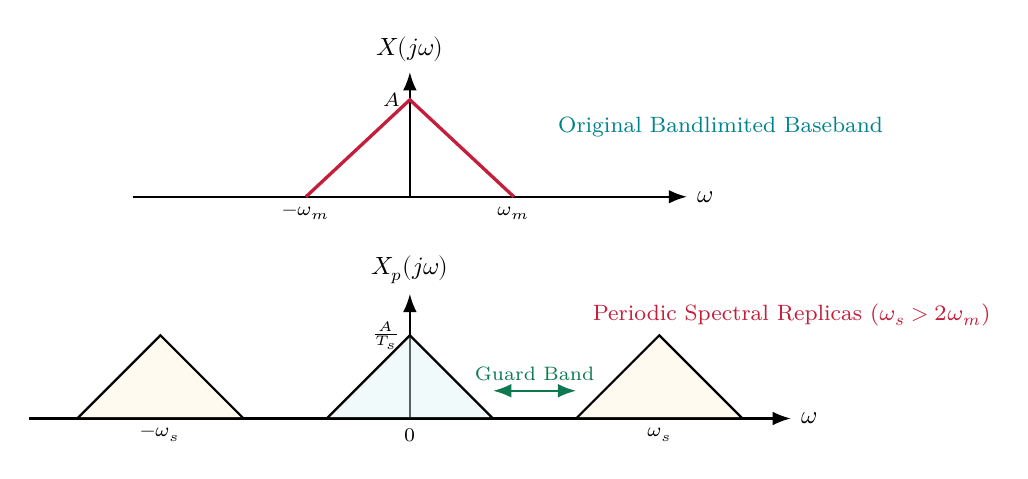
\begin{tikzpicture}[>=Latex, scale=0.88, font=\small]
  % 1. Continuous Spectrum X(jw)
  \begin{scope}[yshift=3.2cm]
    \draw[->, thick] (-4,0) -- (4,0) node[right] {$\omega$};
    \draw[->, thick] (0,0) -- (0,1.8) node[above] {$X(j\omega)$};
    \draw[very thick, myred] (-1.5,0) -- (0,1.4) -- (1.5,0);
    \node[below] at (-1.5,0) {\scriptsize $-\omega_m$};
    \node[below] at (1.5,0) {\scriptsize $\omega_m$};
    \node[left] at (0,1.4) {\scriptsize $A$};
    \node[right, myteal] at (2,1) {\footnotesize Original Bandlimited Baseband};
  \end{scope}

  % 2. Sampled Spectrum (Over-sampled: ws > 2 wm)
  \begin{scope}[yshift=0cm]
    \draw[->, thick] (-5.5,0) -- (5.5,0) node[right] {$\omega$};
    \draw[->, thick] (0,0) -- (0,1.8) node[above] {$X_p(j\omega)$};
    % Baseband k=0
    \draw[thick, fill=hdrteal, fill opacity=0.4] (-1.2,0) -- (0,1.2) -- (1.2,0) -- cycle;
    \node[below] at (0,0) {\scriptsize $0$};
    % Replica k=1
    \draw[thick, fill=hdramber, fill opacity=0.4] (2.4,0) -- (3.6,1.2) -- (4.8,0) -- cycle;
    \node[below] at (3.6,0) {\scriptsize $\omega_s$};
    % Replica k=-1
    \draw[thick, fill=hdramber, fill opacity=0.4] (-4.8,0) -- (-3.6,1.2) -- (-2.4,0) -- cycle;
    \node[below] at (-3.6,0) {\scriptsize $-\omega_s$};
    % Guard bands
    \draw[<->, mygreen, thick] (1.2,0.4) -- (2.4,0.4) node[midway, above] {\scriptsize Guard Band};
    \node[left] at (0,1.2) {\scriptsize $\frac{A}{T_s}$};
    \node[right, myred] at (2.5,1.5) {\footnotesize Periodic Spectral Replicas ($\omega_s > 2\omega_m$)};
  \end{scope}
\end{tikzpicture}
\end{center}
\end{tcolorbox}

% ───────────────────────────────────────────────────────────────────────────────
\section{Aliasing and Anti-Aliasing Techniques}
% ───────────────────────────────────────────────────────────────────────────────

\subsection{The Aliasing Phenomenon}
When a signal is sampled below the Nyquist rate ($\omega_s < 2\omega_m$), the adjacent spectral replicas overlap:
\begin{equation}
  \omega_s - \omega_m < \omega_m \implies \omega_s < 2\omega_m
\end{equation}
In the overlap regions, spectral components from high-frequency replicas fold into the baseband:

\begin{tcolorbox}[defbox, title={\textbf{Definition: Aliasing}}]
\textbf{Aliasing} is the spectral distortion phenomenon whereby high-frequency components of a continuous-time signal fold back across the Nyquist frequency ($f_s / 2$) and appear masquerading as indistinguishable lower-frequency components in the sampled signal.
\end{tcolorbox}

\begin{tcolorbox}[examplebox, title={\textbf{Demonstration: Aliased Frequency of a Sinusoid}}]
Consider a continuous sinusoidal tone $x(t) = \cos(2\pi f_0 t)$ sampled at rate $f_s$:
\begin{equation*}
  x[n] = x(n T_s) = \cos(2\pi f_0 n / f_s)
\end{equation*}
If $f_0 = 70\text{ Hz}$ and $f_s = 100\text{ Hz}$ (where Nyquist frequency is $f_s/2 = 50\text{ Hz}$):
\begin{align*}
  x[n] &= \cos\left(2\pi \frac{70}{100} n\right) = \cos(1.4\pi n) = \cos((2\pi - 0.6\pi) n) \\
  &= \cos(-0.6\pi n) = \cos(0.6\pi n) = \cos\left(2\pi \frac{30}{100} n\right)
\end{align*}
The 70~Hz signal appears identically as an apparent $30\text{ Hz}$ tone ($|f_0 - f_s| = |70 - 100| = 30\text{ Hz}$). The true high-frequency information is irrevocably corrupted.
\end{tcolorbox}

\subsection{Prevention of Aliasing: Anti-Aliasing Filter (AAF)}
Once aliasing occurs, the overlapping spectral components sum together linearly and \textbf{cannot be separated} by any post-processing algorithm. To prevent aliasing:
\begin{enumerate}[topsep=2pt, itemsep=2pt]
  \item \textbf{Pre-Filtering (Anti-Aliasing Filter):} An analog low-pass filter is inserted strictly \textit{before} the sampler. The filter has a cutoff frequency $f_c \le f_s / 2$, suppressing any input spectral energy exceeding the Nyquist foldover limit.
  \item \textbf{Over-sampling:} Selecting $f_s$ significantly higher than $2f_m$ widens the transition band for the analog anti-aliasing filter, allowing lower-order, cost-effective analog filter designs.
\end{enumerate}

% ───────────────────────────────────────────────────────────────────────────────
\section{Signal Reconstruction from Samples}
% ───────────────────────────────────────────────────────────────────────────────

\subsection{The Ideal Reconstruction Filter (Whittaker-Shannon Interpolation)}
When $\omega_s \ge 2\omega_m$, the original spectrum $X(j\omega)$ can be extracted from $X_p(j\omega)$ using an ideal low-pass filter with cutoff frequency $\omega_c$ ($\omega_m < \omega_c < \omega_s - \omega_m$) and gain $T_s$:
\begin{equation}
  H_r(j\omega) = \begin{cases} T_s, & |\omega| \le \frac{\omega_s}{2} \\ 0, & |\omega| > \frac{\omega_s}{2} \end{cases}
\end{equation}
The impulse response $h_r(t)$ of this ideal reconstruction filter is:
\begin{equation}
  h_r(t) = \mathcal{F}^{-1}\{H_r(j\omega)\} = \frac{T_s}{2\pi} \int_{-\omega_s/2}^{\omega_s/2} e^{j\omega t} d\omega = \frac{T_s}{2\pi} \left[ \frac{e^{j\omega t}}{jt} \right]_{-\pi/T_s}^{\pi/T_s} = \frac{\sin(\pi t / T_s)}{\pi t / T_s} = \text{sinc}\left(\frac{t}{T_s}\right)
\end{equation}
Convolving the sampled impulse train $x_p(t)$ with $h_r(t)$ yields:

\begin{tcolorbox}[formulabox, title={\textbf{Whittaker-Shannon Cardinal Reconstruction Formula}}]
\begin{equation}
  x(t) = x_p(t) * h_r(t) = \sum_{n=-\infty}^{\infty} x(n T_s) \text{sinc}\left(\frac{t - n T_s}{T_s}\right)
\end{equation}
where $\text{sinc}(u) \triangleq \frac{\sin(\pi u)}{\pi u}$.
\end{tcolorbox}

\textbf{Geometric Interpolation Property:}
At the exact sampling instants $t = m T_s$:
\begin{equation}
  \text{sinc}\left(\frac{m T_s - n T_s}{T_s}\right) = \text{sinc}(m - n) = \begin{cases} 1, & m = n \\ 0, & m \ne n \end{cases}
\end{equation}
Thus, at each sampling point, the reconstructed signal equals the exact sample value $x(m T_s)$ because all neighboring sinc interpolation curves pass through zero.

\textbf{Practical Limitation:} The ideal sinc interpolator is \textbf{physically unrealizable} because $\text{sinc}(t/T_s)$ has infinite duration, requiring knowledge of all past and future samples ($h_r(t) \ne 0$ for $t < 0$, non-causal).

\subsection{Zero-Order Hold (ZOH)}
In practical digital-to-analog converters (DACs), the simplest and most ubiquitous hold device is the \textbf{Zero-Order Hold (ZOH)}, which clamps each sample value until the arrival of the next sample:
\begin{equation}
  x_{zoh}(t) = x(n T_s) \quad \text{for } n T_s \le t < (n+1)T_s
\end{equation}

\begin{itemize}[topsep=2pt, itemsep=2pt]
  \item \textbf{Impulse Response:} A causal rectangular pulse of duration $T_s$:
  \begin{equation}
    h_0(t) = u(t) - u(t - T_s) = \text{rect}\left(\frac{t - T_s/2}{T_s}\right)
  \end{equation}
  \item \textbf{Frequency Response:}
  \begin{equation}
    H_0(j\omega) = \int_0^{T_s} e^{-j\omega t} dt = \frac{1 - e^{-j\omega T_s}}{j\omega} = T_s \left( \frac{\sin(\omega T_s / 2)}{\omega T_s / 2} \right) e^{-j\omega T_s / 2} = T_s \text{sinc}\left(\frac{\omega T_s}{2\pi}\right) e^{-j\omega T_s / 2}
  \end{equation}
  \item \textbf{Distortion Effects of ZOH:}
  \begin{enumerate}[topsep=2pt, itemsep=2pt]
    \item \textit{In-band Droop (Sinc Roll-off):} Magnitude response attenuates at the band edge $\omega_s/2$ by a factor of $\text{sinc}(0.5) = \frac{2}{\pi} \approx 0.637$ ($-3.92\text{ dB}$).
    \item \textit{High-Frequency Images:} The sinc side-lobes decay slowly ($\propto 1/\omega$), leaving residual harmonic images. A post-reconstruction smoothing filter and equalization circuit ($\frac{1}{\text{sinc}}$) are required.
  \end{enumerate}
\end{itemize}

\subsection{First-Order Hold (FOH)}
The \textbf{First-Order Hold (FOH)} performs linear extrapolation/interpolation between consecutive sample points.
\begin{itemize}[topsep=2pt, itemsep=2pt]
  \item \textbf{Impulse Response (Triangular Pulse):}
  \begin{equation}
    h_1(t) = \begin{cases} 1 - \frac{|t|}{T_s}, & |t| \le T_s \\ 0, & |t| > T_s \end{cases}
  \end{equation}
  \item \textbf{Frequency Response:}
  \begin{equation}
    H_1(j\omega) = T_s \left( \frac{\sin(\omega T_s / 2)}{\omega T_s / 2} \right)^2 = T_s \text{sinc}^2\left(\frac{\omega T_s}{2\pi}\right)
  \end{equation}
  \item \textbf{Advantage:} The side-lobes decay as $1/\omega^2$, providing vastly superior suppression of spectral images compared to ZOH. (A causal implementation requires 1 sample delay $T_s$).
\end{itemize}

% ───────────────────────────────────────────────────────────────────────────────
\section{Relation Between Continuous and Discrete-Time Systems}
% ───────────────────────────────────────────────────────────────────────────────

\subsection{Mapping of Time and Frequency Variables}
When a continuous signal $x_c(t)$ is sampled with period $T_s$, the discrete-time sequence is $x[n] = x_c(n T_s)$. The independent variables are related by:
\begin{equation}
  t = n T_s = \frac{n}{f_s}
\end{equation}
The relationship between continuous-time angular frequency $\omega$ (rad/s) and discrete-time angular frequency $\Omega$ (rad/sample) is:
\begin{equation}
  \Omega = \omega T_s = \frac{\omega}{f_s} = 2\pi \frac{f}{f_s}
\end{equation}

\textbf{Key Frequency Correspondence:}
\begin{itemize}[topsep=2pt, itemsep=2pt]
  \item Continuous DC ($\omega = 0$) maps to Discrete DC ($\Omega = 0$).
  \item Continuous Nyquist frequency ($\omega = \omega_s / 2 = \pi / T_s$) maps directly to the discrete half-sample frequency $\Omega = \pi$.
  \item Sampling frequency $\omega = \omega_s$ maps to $\Omega = 2\pi$ (which is identical to $0$ due to $2\pi$-periodicity).
\end{itemize}

\subsection{Digital Processing of Continuous-Time Signals}
A standard digital signal processing (DSP) system architecture comprises:
\begin{equation*}
  x_c(t) \xrightarrow{\text{AAF}} x_a(t) \xrightarrow{\text{C/D}} x[n] \xrightarrow{\boxed{H(e^{j\Omega})}} y[n] \xrightarrow{\text{D/C}} y_c(t)
\end{equation*}
If sampling satisfies the Nyquist condition ($f_s \ge 2 f_m$), the overall continuous-time system behaves as an equivalent LTI analog filter with effective frequency response:
\begin{equation}
  H_{eff}(j\omega) = \begin{cases} \left. H(e^{j\Omega}) \right|_{\Omega = \omega T_s}, & |\omega| < \frac{\pi}{T_s} \\ 0, & |\omega| \ge \frac{\pi}{T_s} \end{cases}
\end{equation}

% ───────────────────────────────────────────────────────────────────────────────
% QUICK REVISION PAGE
% ───────────────────────────────────────────────────────────────────────────────
\newpage
\begin{center}
  {\Large\bfseries\color{myred} Quick Revision \& Examination Compendium}\\[3pt]
  {\small\color{watermark}\textbf{Module 5: The Sampling Theorem \& Signal Reconstruction}}
\end{center}
\vspace{-2pt}
\noindent{\color{myred}\rule{\linewidth}{0.8pt}}

\begin{tcolorbox}[formulabox, title={\textbf{Key Formulas at a Glance}}]
\par\vspace{4pt}\noindent
\begingroup
\setlength{\tabcolsep}{5pt}
\setlength{\extrarowheight}{3pt}
\renewcommand{\arraystretch}{1.4}
\begin{tabularx}{\linewidth}{|B{4.5cm}|Y|}
\hline
\textbf{Concept / Law} & \textbf{Definitive Mathematical Formula} \\
\hline
Nyquist Sampling Criterion & $f_s \ge 2 f_m \iff \omega_s \ge 2 \omega_m$ \\
\hline
Nyquist Rate & $f_N = 2 f_m \quad (\text{Hz}), \quad \omega_N = 2 \omega_m \quad (\text{rad/s})$ \\
\hline
Nyquist Interval & $T_N = \frac{1}{2 f_m} = \frac{\pi}{\omega_m} \quad (\text{seconds})$ \\
\hline
Sampled Spectrum Replication & $X_p(j\omega) = \frac{1}{T_s} \sum_{k=-\infty}^{\infty} X\big(j(\omega - k \omega_s)\big)$ \\
\hline
Aliased Frequency & $f_{apparent} = |f_0 - k f_s| \le \frac{f_s}{2}$ \\
\hline
Ideal Sinc Interpolation & $x(t) = \sum_{n=-\infty}^{\infty} x(n T_s) \text{sinc}\left(\frac{t - n T_s}{T_s}\right)$ \\
\hline
Zero-Order Hold Transfer Function & $H_0(j\omega) = T_s \left(\frac{\sin(\omega T_s / 2)}{\omega T_s / 2}\right) e^{-j\omega T_s / 2}$ \\
\hline
First-Order Hold Transfer Function & $H_1(j\omega) = T_s \text{sinc}^2\left(\frac{\omega T_s}{2\pi}\right)$ \\
\hline
CT to DT Frequency Mapping & $\Omega = \omega T_s = \frac{\omega}{f_s}$ \\
\hline
Effective DSP Frequency Response & $H_{eff}(j\omega) = H(e^{j\omega T_s}) \quad \text{for } |\omega| < \frac{\pi}{T_s}$ \\
\hline
\end{tabularx}
\endgroup
\end{tcolorbox}

\begin{tcolorbox}[defbox, title={\textbf{One-Line Definitions for Rapid Review}}]
\par\vspace{4pt}\noindent
\begingroup
\setlength{\tabcolsep}{5pt}
\setlength{\extrarowheight}{3pt}
\renewcommand{\arraystretch}{1.35}
\begin{tabularx}{\linewidth}{|B{4.2cm}|Y|}
\hline
\textbf{Term} & \textbf{Definitive Technical Meaning} \\
\hline
Sampling Theorem & Principle stating a bandlimited signal can be perfectly recovered if sampled at $\ge 2\times$ maximum frequency. \\
\hline
Nyquist Rate & The minimum theoretical sampling frequency ($2f_m$) required to avoid spectral overlap and aliasing. \\
\hline
Aliasing & An irreversible distortion where high frequencies fold into lower bands due to inadequate sampling rates. \\
\hline
Anti-Aliasing Filter & An analog low-pass pre-filter that removes signal content above $f_s/2$ prior to sampling. \\
\hline
Whittaker-Shannon Interpolation & The mathematically exact reconstruction formula using weighted, time-shifted sinc functions. \\
\hline
Zero-Order Hold (ZOH) & A DAC reconstruction filter that holds each sample amplitude flat over the entire sampling interval. \\
\hline
First-Order Hold (FOH) & A reconstruction filter that performs linear triangular interpolation between consecutive sample points. \\
\hline
Guard Band & The frequency separation gap $(\omega_s - 2\omega_m)$ between adjacent spectral replicas in over-sampled systems. \\
\hline
Anti-Imaging Filter & A post-DAC analog smoothing filter designed to suppress high-frequency periodic images from the hold circuit. \\
\hline
\end{tabularx}
\endgroup
\end{tcolorbox}

\begin{tcolorbox}[exambox, title={\textbf{Frequently Asked / Viva Questions}}]
\begin{enumerate}[topsep=0pt, label=\textbf{Q\arabic*.}, itemsep=5pt]
  \item \Q{What is the Nyquist rate for the composite signal $x(t) = 3\cos(100\pi t) + 2\sin(300\pi t) - 5\cos(200\pi t)$?}
  Identify the angular frequencies: $\omega_1 = 100\pi \implies f_1 = 50\text{ Hz}$, $\omega_2 = 300\pi \implies f_2 = 150\text{ Hz}$, $\omega_3 = 200\pi \implies f_3 = 100\text{ Hz}$. The highest frequency is $f_m = 150\text{ Hz}$. Thus, Nyquist rate $f_N = 2 f_m = 2 \times 150 = 300\text{ Hz}$ (or $\omega_N = 600\pi\text{ rad/s}$).

  \item \Q{What is the Nyquist rate for $x(t) = \text{sinc}(100 t) \cdot \text{sinc}(200 t)$?}
  In the frequency domain, multiplication in time corresponds to convolution: $X(j\omega) = \frac{1}{2\pi} [X_1(j\omega) * X_2(j\omega)]$. The bandwidths of the rectangular spectra add: $W = W_1 + W_2 = 100\pi + 200\pi = 300\pi\text{ rad/s}$. Thus, $f_m = 150\text{ Hz}$, giving Nyquist rate $f_N = 2 f_m = 300\text{ Hz}$.

  \item \Q{Why cannot an aliased signal be corrected or de-aliased digitally after sampling?}
  Once aliasing occurs, overlapping high- and low-frequency spectral components sum together into identical frequency bins in the sampled sequence. Since a single composite sum contains no tag indicating individual source components, separation is mathematically impossible.

  \item \Q{Why is an Anti-Aliasing Filter placed before the sampler rather than after?}
  Because aliasing occurs during the sampling operation itself. Placing the filter after the sampler attempts to filter a signal that is already contaminated with folded noise that now resides in the legitimate signal band.

  \item \Q{Why is ideal sinc interpolation practically unrealizable?}
  Because $\text{sinc}(t/T_s) = \frac{\sin(\pi t / T_s)}{\pi t / T_s}$ has infinite duration extending from $t = -\infty$ to $+\infty$. Realizing it would require infinite delay and infinite non-causal memory.

  \item \Q{What is the passband droop caused by a Zero-Order Hold (ZOH)?}
  The ZOH frequency response has magnitude $|H_0(j\omega)| = T_s \left|\frac{\sin(\omega T_s / 2)}{\omega T_s / 2}\right|$. At the band edge $\omega = \omega_s / 2$, $|H_0| = T_s \frac{\sin(\pi/2)}{\pi/2} = \frac{2}{\pi} T_s \approx 0.637 T_s$. This produces an in-band attenuation of $20\log_{10}(2/\pi) \approx -3.92\text{ dB}$, requiring an inverse-sinc equalizer.

  \item \Q{Compare ZOH and FOH in terms of spectral image suppression.}
  ZOH has side-lobes that decay at a rate of $1/\omega$ ($-20\text{ dB/decade}$), whereas FOH has side-lobes that decay at $1/\omega^2$ ($-40\text{ dB/decade}$). FOH provides vastly superior attenuation of high-frequency images.

  \item \Q{What continuous frequency $\omega$ corresponds to $\Omega = \pi$ in a discrete-time system?}
  $\Omega = \omega T_s = \pi \implies \omega = \frac{\pi}{T_s} = \frac{\omega_s}{2} = \pi f_s$. This corresponds precisely to the continuous-time Nyquist foldover frequency.

  \item \Q{What is meant by flat-top sampling and how does it differ from natural sampling?}
  In natural sampling, the tops of the sampled pulses follow the exact analog contour of $x(t)$. In flat-top sampling, each pulse has a constant (flat) amplitude equal to the sample value at the pulse onset. Flat-top sampling introduces aperture distortion ($\text{sinc}$ attenuation) similar to a sample-and-hold circuit.

  \item \Q{What is the Nyquist rate for $x(t) = \cos^2(400\pi t)$?}
  Using the trigonometric identity: $\cos^2(\theta) = \frac{1 + \cos(2\theta)}{2}$. Thus, $x(t) = \frac{1}{2} + \frac{1}{2}\cos(800\pi t)$. The maximum frequency is $f_m = 400\text{ Hz}$. Hence, the Nyquist rate is $f_N = 2 f_m = 800\text{ Hz}$.
\end{enumerate}
\end{tcolorbox}

\begin{tcolorbox}[tikzbox, title={\textbf{Summary Matrix: Comparison of Signal Reconstruction Methods}}]
\par\vspace{4pt}\noindent
\begingroup
\setlength{\tabcolsep}{4.5pt}
\setlength{\extrarowheight}{3pt}
\renewcommand{\arraystretch}{1.35}
\begin{tabularx}{\linewidth}{|B{3.2cm}|B{3.8cm}|B{3.2cm}|Y|}
\hline
\textbf{Reconstruction Filter} & \textbf{Impulse Response $h(t)$} & \textbf{Frequency Response} & \textbf{Practical Feasibility} \\
\hline
Ideal Sinc Interpolator & $\text{sinc}(t / T_s)$ & Ideal brick-wall boxcar & Unrealizable; non-causal, infinite delay. \\
\hline
Zero-Order Hold (ZOH) & $\text{rect}\left(\frac{t - T_s/2}{T_s}\right)$ (Staircase) & $T_s \text{sinc}\left(\frac{\omega T_s}{2\pi}\right) e^{-j\omega T_s/2}$ & Universal in DACs; causes $-3.92\text{ dB}$ droop. \\
\hline
First-Order Hold (FOH) & $\text{tri}\left(\frac{t}{T_s}\right)$ (Linear interpolation) & $T_s \text{sinc}^2\left(\frac{\omega T_s}{2\pi}\right)$ & Causal with 1 sample delay; $-40\text{ dB/dec}$ rolloff. \\
\hline
\end{tabularx}
\endgroup
\end{tcolorbox}

\end{document}
